\chapter{Introduction}\label{chap:introduction}
 
 Ray Kurzweil said that Artificial intelligence will reach human levels by the year 2045 at Forbes and the current pace of the field's progress proves it, especially during the past few decades. The main reason behind this is Machine Learning, a branch of AI that deals with teaching computers how to learn rather than how to perform is the reason for this incredible change. This necessity of teaching computers to think like human lead to the invention of Artificial Neural Networks typically called as ANNs. Deep Learning is a subfield of machine learning that deals with these ANNs. Now as the name suggests an ANN is a computational model which was developed by the magical combination of biology, mathematics and computer science. Biology because they are inspired by the way our brain processes the information. These networks make use of data that they have access to and make predictions from them through the iteration process. In recent times they have provided solutions to many problems in computer vision, speech recognition and natural language processing.
 \section{Definition of a Neural Network}
 \setlength{\parindent}{10ex}
 Neural Network can be defined as the highly interconnected system that endeavors to recognize the underlying relationship between data through a process that simulates the way human brain operates. They can adapt to the changing input so the network generates the best possible result without needing to redesign the output criteria.\underline{spoorti} %\cite{IEEE485891}
 
 The basic unit of computation in Neural Network is a neuron which is referred to as a node. And all these nods are connected through synapses through which the information flows. Each node receives input from other node or external source and computes the output with the help of their assigned weights. When we train this neural network with the data each neuron fires whenever it learns a particular pattern from the data and this firing rate is modeled using an activation function. The process of computing the output at each neuron can be mathematically represented as given in \textit{figure 1.1}


\begin{figure}
    \centering
    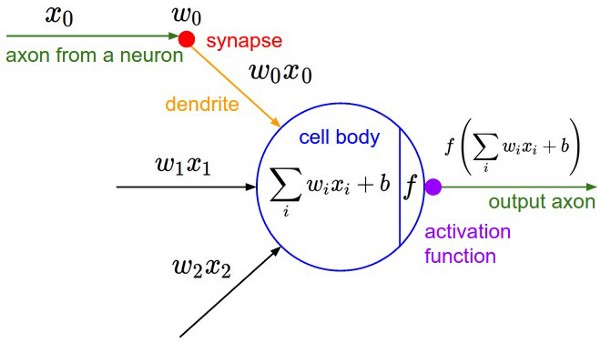
\includegraphics[width=0.5\textwidth]{thesis_template/images/Mathmodel.png}
    \caption{Mathematical representation of a neuron}
    \label{}
    \source{\url{http://cs231n.github.io/convolutional-networks/}}
\end{figure}


 Here the node takes numerical inputs $\mathit{x_0,x_1}$ and  $\mathit{x_2}$ which are assigned with weights $\mathit{w_1,w_2,w_2}$ respectively and calculates the output with the help of a non-linear function \textit{f} which is known as activation function. The main idea behind introducing the activation function is to make the network learn non-linear representations as most of the data in the real world is non-linear. And the Bias \textit{b} decides whether the neuron should fire or not, in simple terms there is no output without it. Bias provides every node with trainable constants.%\cite{IEEE485891}
\subsubsection{\textbf{Now let us see the structure and working of model}}

The network architecture has three different layers which contain set of nodes, they are referred as
\begin{itemize}
    \item \textbf{Input layer:} This is a layer which is essential in introducing different patterns to the network. It just acts as a bridge between data and the hidden layers and there is no modification of data here.
    \item \textbf{Hidden layers:} They are set of layers where all the computations are done. They perform computations by applying different functions and transfer the output in the form of weights to the next layer which can be another hidden layer or output layer. There can be N number of hidden layers whose main job is to transform the data into something an output layer can use.
    \item \textbf{Output Layer:} It consists of a set of nodes that are responsible for collecting the information from hidden layers and then transmits it according to the way it was designed to give to the outside world. And the pattern represented by the output layer can be traced back to the input layer.
\end{itemize}


\begin{figure}
    \centering
    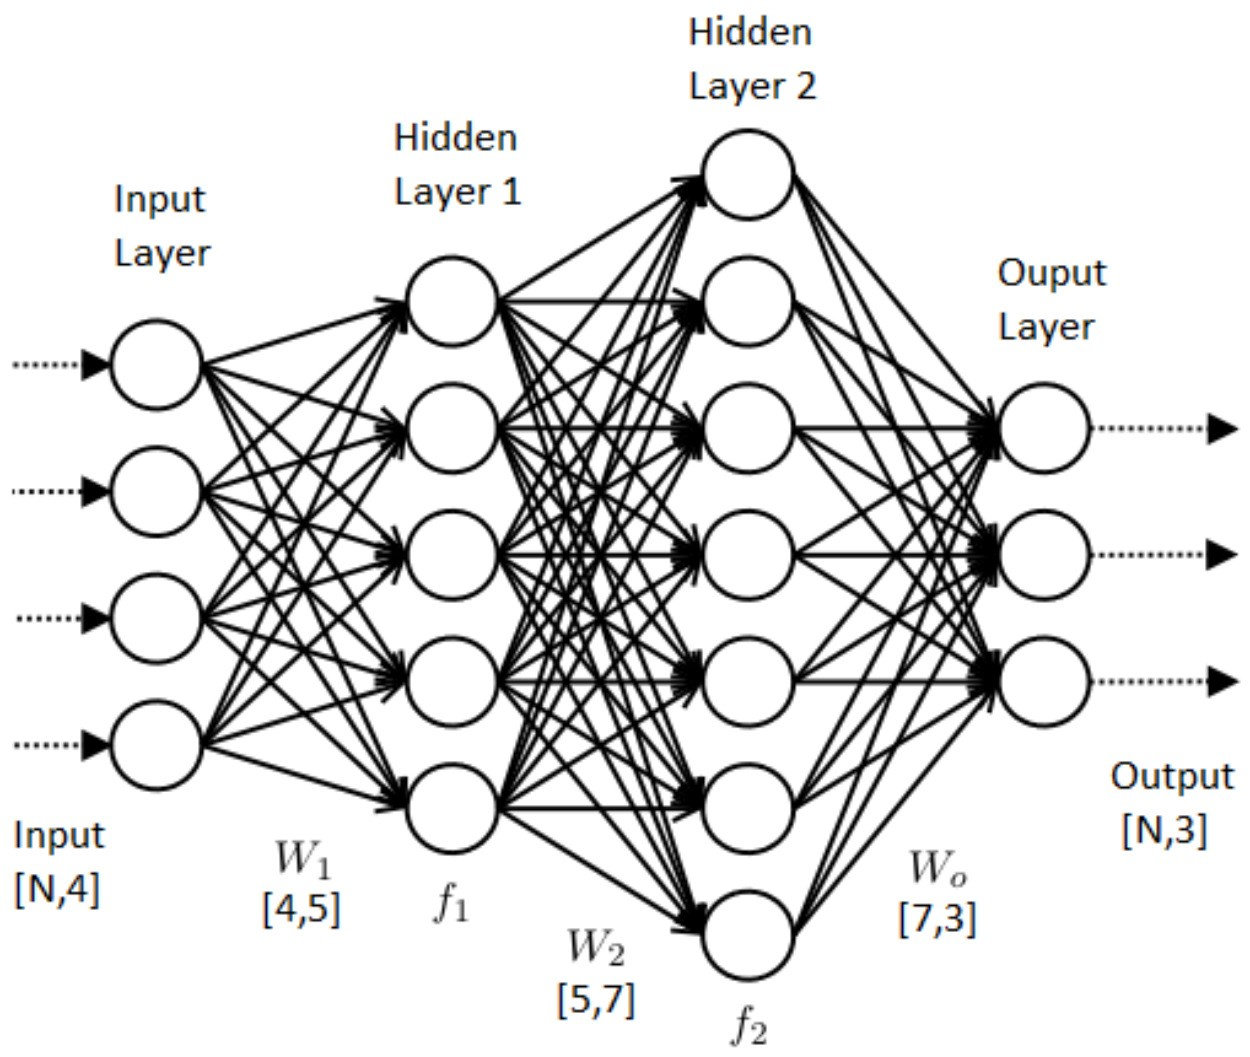
\includegraphics[width=0.5\textwidth]{thesis_template/images/ANN.png}
    \caption{A simple Neural Network}
    \label{}
    \source{\url{https://medium.com/coinmonks/the-artificial-neural-networks-handbook-part-1-f9ceb0e376b4}}
\end{figure}
\noindent The figure represents the basic architecture of a \textit{\textbf{feedforward}} neural network where data enters at the input layers and continues to pass through the network layer by layer where classification is done. There is no feedback between the layers and hence it is called a feedforward network. In an NN output of one layer is the input of another layer.
\subsection{Learning process of Neural Networks}
As mentioned above Neural Networks are about learning from the data and making predictions based on it. Most widely used learning technique is \textit{Supervised Learning} where the input data is already assigned with output labels. The learning process involves different phases as described below
\begin{itemize}
    \item \textbf{Defining Model:} Building the model with random initialization of weights is a very common practice. And later on, through an iterative learning process, the weights can be updated in order to get the ideal model which has the best prediction.
      \item \textbf{Forward pass:} The next step after initializing the model is to check its performance. We start by passing the input we have through the model and calculate the actual output of the model straightforwardly. As the data is flowing in the forward direction it is known as forward pass.
 
     \item \textbf{Calculating the loss function:} By this step, we have actual output calculated by the model but we already have desired output which we want network to learn. In order to achieve it, we first need to calculate Loss, Error or Cost function which is the difference between actual output and desired output.
     $$E(w)= p - p^* $$
     where E is the cost function and \textit{p} is the desired output and $p^* $ is the actual output. Different loss functions calculate different error rates for the same predictions thus it has a considerable amount of effect on the model. Most commonly used loss function is Mean Squared Error which calculates the square of the difference between actual value and the predicted value.
     $$MSE = \frac{1}{2}\sum{(f_i- y_i)^2}$$
     where $f_i$ is the predicted output and $y_i$ is the desired output. The value of this loss function is inversely proportional to the performance of the model.
     \item \textbf{Learning process:} After calculating the error function E(w) we now focus on optimizing the weights in the model which is done by learning algorithm known as \textbf{\textit{Backpropagation}}. It is a first-order iterative optimization algorithm for finding the local/global minima of a cost function. Backpropagation works by calculating the partial derivative of the loss function w.r.t weights at a particular layer $\frac{\partial E(w)}{\partial w}$ applying chain rule in calculus.%\cite{IEEE118638}
    \begin{figure}
    \centering
    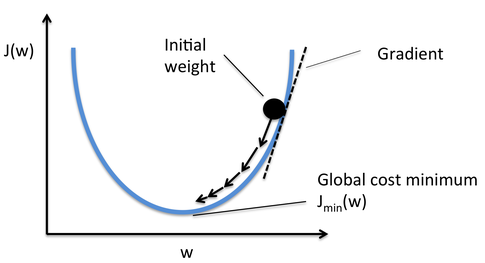
\includegraphics[width=0.6\textwidth]{thesis_template/images/backprop.png}
    \caption{Backpropagation curve}
    \label{}
    \source{\url{https://medium.com/datathings/neural-networks-and-backpropagation-explained-in-a-simple-way-f540a3611f5e}}
    \end{figure}
     
    
    \noindent Basically backpropagation focuses only on calculating the gradients and gives you the direction in which you minimize the error. But updating these weights can be handled using different optimization techniques like gradient descent,stochastic gradient descent or Adam optimizer. The updated weight is
    $$w_1 = w_0 -  \alpha . \frac{\partial E(w)}{\partial w} $$
    
\newpage\noindent In the above formula $w_1$ is updated weight, $w_0 $ is an old weight, $\frac{\partial E(w)}{\partial w}$ is gradient of loss function w.r.t $w_0 $ and $\alpha $ is learning rate a hyperparameter which is randomly given by the user to control the adjusting of weights. The learning rate should not be too low nor too high in order to make sure that we are not missing the local minima.
     \end{itemize}
     This is the common learning process of a Neural Network\cite{IEEE118638}. Now coming to the special kind of Neural network called Convolutional Neural Network which is the type of ANN used in this thesis.
    \subsection{An Intuitive Introduction to Convolutional Neural Networks}
    A specific kind of deep neural networks is Convolutional Neural Network commonly referred to as CNN or Convnet. Inspired by the research of D.H.Hubel and T.N.Wiesel in the 1950s and 1960s which suggested a new model for how mammals visually perceive the world Convolutional Neural Networks are developed. These models belong to a class of ANNs that are designed specially to analyze visual imagery. %\cite{lecun}
    
    Generally, it is very complex to flatten the image and feed it to the normal Neural Network as it requires a large amount of parameters to define this kind of network. Therefore CNNs are proposed to solve tasks related to visual analysis. Unlike regular ANNs where each and every neuron of one layer is connected to other layer, CNNs have a different structure. Firstly the layers are arranged in \textbf{3 dimensions:width,height and depth}. Next, the neurons in one layer do not connect to all the neurons in the next layer but only a small region of it is connected because it will be computationally very expensive if all the neurons are connected. Lastly, the final output will be reduced to a single vector of probability scores which is organized along the depth dimension. This probability score decides the class of an image%\cite{OSheaN15}. The structure is shown in \textit{figure 1.4}
    
     
      \subsubsection{Convnets have two parts}
     \begin{itemize}
      \item \textit{\textbf{Feature extraction}}, which is performed in hidden layers where different patterns/features are learned from the given input image.
      \item \textit{\textbf{Classification}}, involves few fully connected layers which serve as a classifier for the extracted features. They assign a probability for the object on the image.
         
     \end{itemize}
     \subsubsection{\textbf{Architecture of CNN:}}
   
      \begin{figure}[h]
    \centering
    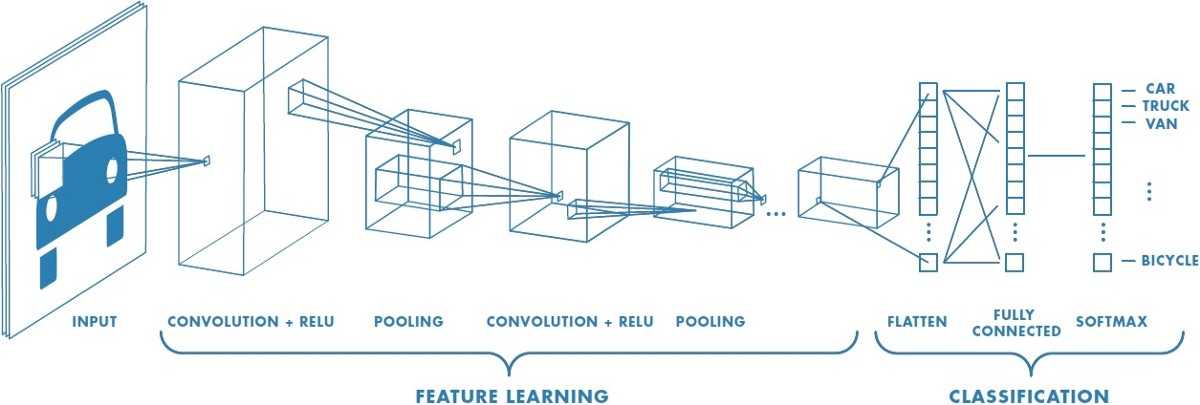
\includegraphics[width=1\textwidth]{thesis_template/images/CNN.jpeg}
    \caption{Structure of a CNN }
    \label{}
    \source{\url{https://www.mathworks.com/videos/introduction-to-
    deep-learning-what-are-convolutional-neural-networks--1489512765771.html}}
    \end{figure}
 \newpage  \subsubsection{\textbf{Working of the network:}}
     When we feed the network with input image the following operations are performed sequentially by the network:
\begin{itemize}
    \item \textbf{Convolution Layer:} Convolution generally means merging of two things to produce a different thing. Most of the heavy computations are done at this layer. The layer consists of a set of learnable \textit{filters or kernels or weights} each learning to look for something different in an image. And during the forward pass, each filter is slid across the width and height of the input to produce an activation map. Numerous convolutions are performed here as each filter is convolved only with a small region of input and this results in many activation maps. All these maps are put together as a final output of the layer.%\cite{8308186}
    
   The layer also consists of two hyperparameters that control the output volume or their spatial arrangement. Firstly we must specify \textit{\textbf{Stride}}, it is the size of the step the convolution filter moves each time. For example, if the stride value is 1 it means that the filter moves pixel by pixel. The larger stride results in the smaller output volumes spatially.\cite{8308186}
   
 \setlength{\parindent}{10ex} Secondly,\textit{\textbf{Zero-padding}} which means the addition of zero value pixels surrounding the input image. Because the feature map is always smaller than the input this is done in order to prevent it from shrinking. Doing so also helps in increasing the performance of the model.\cite{8308186}
 \item \textbf{Activation layer:} Activation functions help Artificial Neural Network to learn and make sense of something really complicated and Non-linear complex functional mappings between the inputs and output variable. This layer determines the output of the filter i.e., whether it should fire or not. The activation function is always non-linear in order to make it easy for the model to generalize or adapt to a wide variety of data. The non-linear function graph is represented as below.
 \begin{figure}[h]
    \centering
    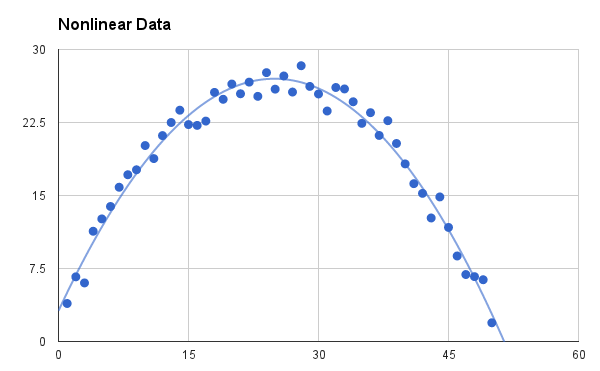
\includegraphics[width=0.5\textwidth]{thesis_template/images/nonlinear.png}
    \caption{Non-linear graph}
    \label{}
    \source{\url{https://towardsdatascience.com/activation-functions-neural-networks-1cbd9f8d91d6}}
    \end{figure}
 
 
 \newpage\noindent There are so many activation functions like \textit{\textbf{Sigmoid}}, \textit{\textbf{Tanh}} but  \textbf{\textit{ReLU}} is the most commonly used activation function  by CNN just like any other Neural Network to produce non-linear output. This layer maps the function $f(x) = max(0,x) $. This function changes all the negative outputs to zero. It is very important as negative values also contribute to the output of the next layers which means the absence of the feature. But it does not have any effect on the shape of the image.\cite{8308186} 
 \item\textbf{Pooling Layer:} Image processing is a very computationally intensive process. In order to allow our model to run at a decent speed while not compromising on accuracy too heavily, we do a form of dimension reduction on the image size in a technique called pooling. It is very important to have a pooling layer between two successive convolutional layers whose function is to reduce the spatial size of the representation.\\
 \begin{figure}[h]
    \centering
    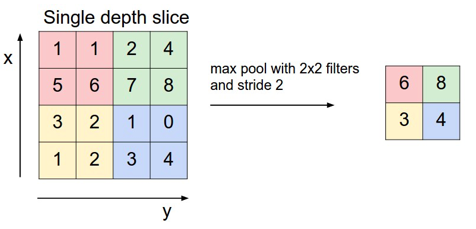
\includegraphics[width=0.5\textwidth]{thesis_template/images/maxpool.png}
    \caption{\small Max-pooling}
    \label{}
    \source{\url{http://cs231n.github.io/convolutional-networks}}
    \end{figure}\\
 The most commonly used pooling is \textbf{\textit{max-pooling}} which considers the maximum value in each window without losing the significant information. This layer reduces the amount of parameters and computations in the network. The most common form of a pooling layer has filters with a size of $2*2 $ with a stride of 2 which discards atleast 70 percent of activations. This layer also works alot like convolutional layer.

  
    
    \item \textbf{Fully-connected Layer:} After the convolution and pooling layers the important task of classification is done by fully-connected layer. The main goal of these layers is to flatten the features that are learned by the convolutional layers. All the neurons in these layers are connected to all the activations in the previous layer and they convert 3D data to 1D data into a set of probabilities. The most commonly used function for the conversion of the data is \textit{softmax function}, it gives the set of discrete probabilities for each class we are trying to predict. It computes the probabilities of each target class over all possible classes. It can be mathematically expressed as follows. 
    $$\sigma(y_i) = \frac{e^{y_i}}{\sum_{j=1}^{N} e^{y_j}}$$
     Where N is the number of classes. Next we use $argmax(\sigma (y_i))$ function to map the input image $x_i$ to its class $y$.\cite{8308186}
    \end{itemize}
    All these steps contribute to one forward pass of an image in the network. The training of a CNN is done using backpropagation gradient descent algorithm.
  
  
  \section{Problem Statement:}
   Ever since their introduction during the early 1990s by Yann LeCun\cite{lecun} Convolutional Neural Networks have been performing very well in tasks related to computer vision and almost reached human-level performance. Especially because of their parameter sharing they can be used in any device. The incredible speed of research in this area combined with the open availability of GPUs and large databases has given impressive results in past few years. Now CNNs are one of the important non-linear models that are used in most devices starting from face recognition in your phone to Google self-driving cars\cite{Al-Qizwini} and they are the go-to model for every image related problem. In terms of performance, they have achieved superhuman accuracy which means that they perform better than humans. 
   
\noindent   Now, the problem with these models is though their performance is very impressive sometimes it is difficult to understand what and how exactly these large models are learning. For this reason, they are often considered as black-box models. And without understanding the internal working of the network it is hard to trust them. For example, let us assume that we are training the network with images of bedroom, now the question is what is the model specifically looking for. It may classify the image just by looking for a bed or lamp or a table, so now next time whenever it detects a table there is a possibility that it classifies the image as bedroom. But it might be an office image, now the model has done wrong classification. The technique to overcome this type of problems is visualization of trained filters. Visualizing the nodes inside the network solved many problems related to these deep models. Lately, there is a lot of research going on in this field of visualizing what is happening inside the network.
  \subsection{Need to Visualize}
   \begin{itemize}
       \item To understand how the model is making these predictions.
       \item To see if parameters and hyperparameters are chosen correctly and if not tune them for obtaining better models.
       \item Ensure if all the filters are learning because in some cases filters might converge to zero which means that they are not really being used.
       \item Also helps in debugging the model.
       \item To tell where the network has been saturated. 
   \end{itemize}
\newpage   \subsection{Research Questions}
   This thesis includes answering the two questions mentioned below:
\begin{itemize}
    \item \textbf{Visualize the hidden layers of the Convolutional Neural Network:}
    
    This includes visualizing the weights of the trained model and also look if different parameters and the hyperparameters have any effect on the learning patterns of the nodes. The main part of this thesis includes only convolutional layers so fully-connected layers are ignored. 
    \item \textbf{Looking for the redundancy in the network:}
    
  We say the network is redundant when two or more filters or layers in the network learn the same pattern. And a redundant network consumes a lot of computation time and effort. The work also includes finding out if there are redundant filters in the network and if so what kind of parameters are causing it. 
\end{itemize}


    

    
     
     
     

     
     
     
     
     
     
     
 






